

\begin{figure}
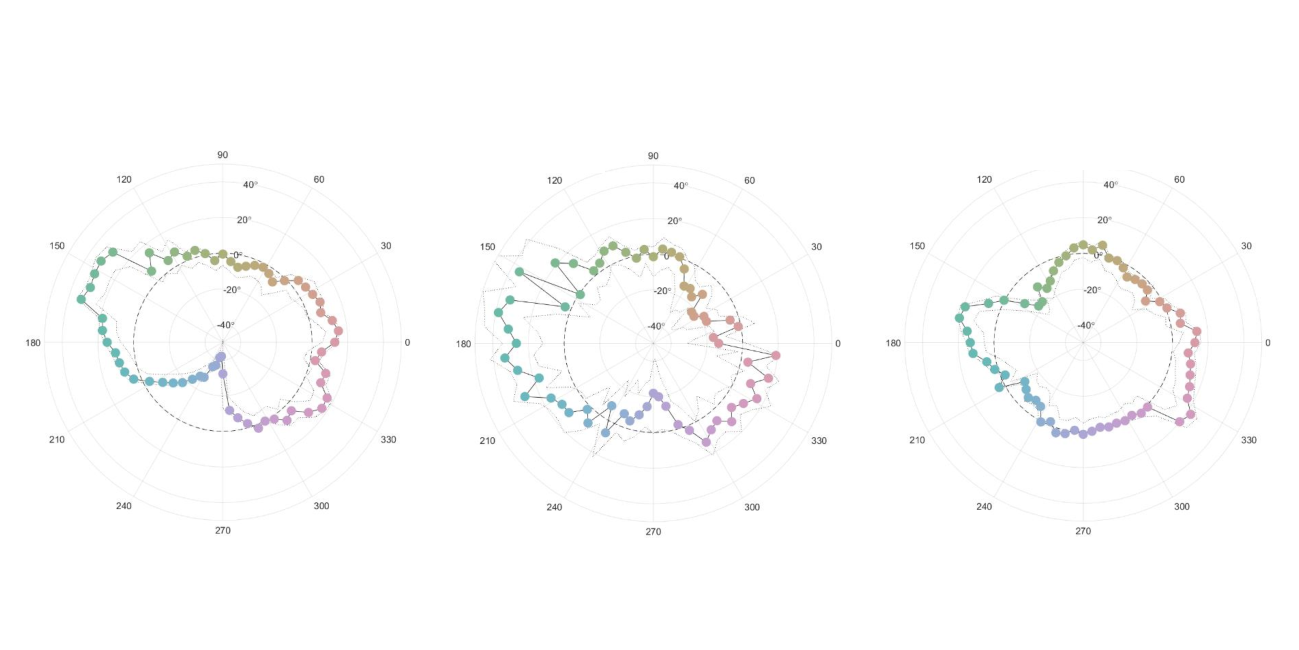
\includegraphics[width=\textwidth]{../../Figures/Old/biasfigs.pdf}
\caption{Bias as a function of hue, for Conway monkeys} 
\end{figure}
\paragraph{Monkeys exhibit hallmarks of colour category behavior}

The key result is that monkeys do show a hallmark of colour categorization behavior - that is: memory biases towards a set of particular points in a colorspace that is defined by perceptual uniformity. 


\paragraph{Shared colour categories across monkeys}

We see that all tested monkeys share two common categories - a warm/orange-ish category, and a cool/blue-ish category.
In the absence of language, we can assume that these shared categories arise either due to innate biological factors, environmental factors such as the distribution of colors in the terrestrial environment, or a combination of the two.
These categories align well with the daylight locus, and also the object/category distinction previously identified.

\paragraph{Individual differences}

In one animal we see evidence of additional categories: strong evidence for a greenish category and weak evidence for a purple category.


\paragraph{Controls for non-uniformity of colorspace}

We (hopefully will) disambiguate biases that arise from residual non-uniformity in the colorspace, and those that arise from memory biases.

It is plausible that there are non-uniformities in CIELUV that may result in our nominally iso-saturated colors actually appearing to have variable saturation. This would be a concern, as it would be a reasonable prediction that higher saturation colors would be more salient, and thus more likely to be selected as responses. In a control experiment we see no (or very little) bias towards higher saturation colors.

% Results table?


\paragraph{Learning rates/DKL}
\paragraph{Limitations of colorspace}
\paragraph{Comparison with humans}
\paragraph{Independent verification of found categories}

\begin{figure}
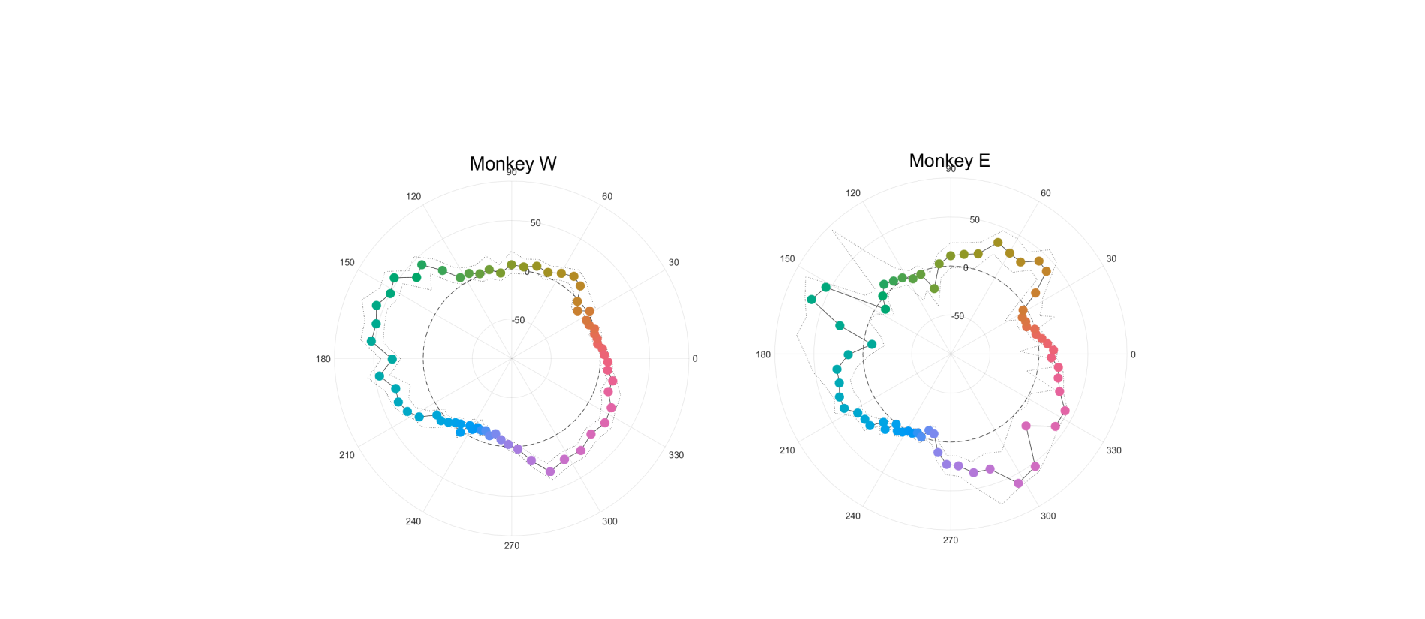
\includegraphics[width=\textwidth]{../../Figures/Old/panichellobias.pdf}
\caption{Bias as a function of hue, for Panichello monkeys} 
\end{figure}


